%%%%%%%%%%%%%%%%%%%%%%%%%%%%%%%%%%%%%%%%%%%%%%%%%%%%%%%%%%%%%%%%%%%%%%%%%%%%%%%
%% SOCIOL 723 -- Social Statistics II
%% Week 9 -- Regression Discontinuity Designs
%% Wenhao Jiang, Duke University, Fall 2026
%%%%%%%%%%%%%%%%%%%%%%%%%%%%%%%%%%%%%%%%%%%%%%%%%%%%%%%%%%%%%%%%%%%%%%%%%%%%%%%

\documentclass[aspectratio=169,11pt,xcolor=dvipsnames]{beamer}
\mode<presentation>

%% ---- fonts: Latin Modern Roman (the LaTeX default), serif throughout -------
\usepackage[T1]{fontenc}
\usepackage{lmodern}
\usefonttheme{serif}
\renewcommand{\familydefault}{\rmdefault}

%% ---- packages --------------------------------------------------------------
\usepackage{amsmath,amsfonts,amssymb,bm}
\usepackage{graphicx}
\usepackage{booktabs}
\usepackage{tikz}
\usetikzlibrary{arrows.meta,positioning,calc}
\usepackage[english]{babel}

\newcommand{\srcp}[1]{{\scriptsize\color{gray}(#1)}}
\newcommand{\srct}[1]{#1}

\DeclareMathOperator*{\argmin}{arg\,min}
\DeclareMathOperator*{\argmax}{arg\,max}
\DeclareMathOperator{\Cov}{Cov}
\DeclareMathOperator{\Var}{Var}
\DeclareMathOperator{\trace}{tr}
\DeclareMathOperator{\rank}{rank}
\DeclareMathOperator{\plim}{plim}
\newcommand{\indep}{\perp\!\!\!\perp}

%% ---- notation conventions (course-wide) ------------------------------------
\newcommand{\E}{E}
\newcommand{\En}{\mathbb{E}_n}
\newcommand{\R}{\mathbb{R}}
\newcommand{\X}{\bm{X}}
\newcommand{\Y}{\bm{y}}
\newcommand{\Ix}{\bm{I}}
\newcommand{\zero}{\bm{0}}
\newcommand{\bhat}{\hat{\bm{\beta}}}
\newcommand{\dto}{\overset{d}{\longrightarrow}}
\newcommand{\pto}{\overset{p}{\longrightarrow}}
\usetikzlibrary{shapes,decorations.pathmorphing}
\newcommand{\lik}{\mathcal{L}}
\newcommand{\loglik}{\ell}
\newcommand{\Info}{\mathcal{I}}
\newcommand{\SE}{\widehat{\text{SE}}}

%% ---- theme -----------------------------------------------------------------
\usetheme{default}
\useoutertheme[subsection=false]{miniframes}
\setbeamertemplate{mini frames}{}

\definecolor{dukeblue}{RGB}{1,33,105}
\definecolor{accent}{RGB}{200,78,0}
\definecolor{softgray}{RGB}{242,242,245}

\setbeamercolor{structure}{fg=dukeblue}
\setbeamercolor{frametitle}{fg=dukeblue,bg=white}
\setbeamercolor{section in head/foot}{fg=white,bg=dukeblue}
\setbeamercolor{alerted text}{fg=accent}
\setbeamercolor{block title}{fg=white,bg=dukeblue}
\setbeamercolor{block body}{fg=black,bg=softgray}
\setbeamercolor{block title alerted}{fg=white,bg=accent}
\setbeamercolor{block body alerted}{fg=black,bg=softgray}

\setbeamertemplate{footline}[page number]
\setbeamertemplate{navigation symbols}{}
\setbeamertemplate{itemize items}[circle]
\setbeamertemplate{blocks}[rounded][shadow=false]
\setbeamerfont{frametitle}{series=\bfseries}
\setbeamerfont{footnote}{size=\scriptsize}
\setbeamerfont{caption}{size=\footnotesize}
\setbeamertemplate{subsection in head/foot}{}
\setbeamertemplate{subsection in head/foot shaded}{}
\setbeamertemplate{caption}[numbered]

\newcommand{\adv}{\,\raisebox{0.6pt}{\textcolor{accent}{$\bigstar$}}}

\setbeamertemplate{section page}{%
  \begin{centering}\vfill
  {\usebeamercolor[fg]{structure}\Large\bfseries\insertsectionhead\par}
  \vskip4pt{\color{dukeblue}\rule{0.35\linewidth}{1pt}\par}
  \vfill\end{centering}}
\setbeamertemplate{subsection page}{%
  \begin{centering}\vfill
  {\usebeamercolor[fg]{structure}\large\bfseries\insertsubsectionhead\par}
  \vfill\end{centering}}

\AtBeginDocument{%
  \setlength{\abovedisplayskip}{5pt}%
  \setlength{\belowdisplayskip}{5pt}%
  \setlength{\abovedisplayshortskip}{2pt}%
  \setlength{\belowdisplayshortskip}{3pt}%
}
\setbeamertemplate{frametitle}{%
  \vskip4pt\usebeamerfont{frametitle}\usebeamercolor[fg]{frametitle}%
  \insertframetitle\par\vskip2pt}
\setbeamersize{text margin left=0.75cm, text margin right=0.75cm}

%% ---- title -----------------------------------------------------------------
\title[SOCIOL 723]{SOCIOL 723: Social Statistics II\\[2pt]}
\subtitle{\large Week 9 --- Regression Discontinuity Designs\\[-8pt]}
\author[Jiang]{\large Wenhao Jiang\vspace{-1.5em}}
\institute[Duke]{}
\titlegraphic{
\includegraphics[height=1.3cm]{../Misc/duke_logo.png}}
\date{\large Department of Sociology, Fall 2026}


\begin{document}

\begin{frame}[plain]
  \titlepage
\end{frame}

\begin{frame}{Today}
  \tableofcontents
\end{frame}

\begin{frame}{The Idea in One Picture}
Many treatments are assigned by a rule: a test score threshold, an income
cut-off, a vote share above 50\%, an age of eligibility.
\vskip2pt
\begin{center}
\begin{tikzpicture}[scale=0.92]
  \draw[->] (0,0) -- (9.4,0) node[right]{\scriptsize running variable $X$};
  \draw[->] (0,0) -- (0,3.1) node[above]{\scriptsize $Y$};
  \draw[gray,dashed,thick] (4.6,0) -- (4.6,3.0);
  \node[gray] at (4.6,-0.35) {\scriptsize cutoff $c$};
  \draw[dukeblue,very thick,smooth,samples=60,domain=0.3:4.55,variable=\x] plot ({\x},{0.7+0.22*\x});
  \draw[accent,very thick,smooth,samples=60,domain=4.65:9.0,variable=\x] plot ({\x},{1.6+0.22*\x});
  \fill[dukeblue] (4.6,1.712) circle (2pt);
  \fill[accent] (4.6,2.612) circle (2pt);
  \draw[<->,thick,black] (4.85,1.712) -- (4.85,2.612);
  \node[right] at (4.95,2.16) {\scriptsize $\tau$};
  \fill[dukeblue!45] (0.60,0.719) circle (1.1pt);
  \fill[dukeblue!45] (0.88,0.670) circle (1.1pt);
  \fill[dukeblue!45] (1.16,1.052) circle (1.1pt);
  \fill[dukeblue!45] (1.44,0.743) circle (1.1pt);
  \fill[dukeblue!45] (1.72,1.101) circle (1.1pt);
  \fill[dukeblue!45] (2.00,1.054) circle (1.1pt);
  \fill[dukeblue!45] (2.28,0.919) circle (1.1pt);
  \fill[dukeblue!45] (2.56,1.268) circle (1.1pt);
  \fill[dukeblue!45] (2.84,1.029) circle (1.1pt);
  \fill[dukeblue!45] (3.12,1.344) circle (1.1pt);
  \fill[dukeblue!45] (3.40,1.173) circle (1.1pt);
  \fill[dukeblue!45] (3.68,1.248) circle (1.1pt);
  \fill[dukeblue!45] (3.96,1.523) circle (1.1pt);
  \fill[dukeblue!45] (4.24,1.842) circle (1.1pt);
  \fill[accent!55] (4.80,2.415) circle (1.1pt);
  \fill[accent!55] (5.10,2.545) circle (1.1pt);
  \fill[accent!55] (5.40,2.870) circle (1.1pt);
  \fill[accent!55] (5.70,3.141) circle (1.1pt);
  \fill[accent!55] (6.00,2.969) circle (1.1pt);
  \fill[accent!55] (6.30,2.920) circle (1.1pt);
  \fill[accent!55] (6.60,3.357) circle (1.1pt);
  \fill[accent!55] (6.90,2.828) circle (1.1pt);
  \fill[accent!55] (7.20,3.413) circle (1.1pt);
  \fill[accent!55] (7.50,3.115) circle (1.1pt);
  \fill[accent!55] (7.80,3.088) circle (1.1pt);
  \fill[accent!55] (8.10,3.137) circle (1.1pt);
  \fill[accent!55] (8.40,3.325) circle (1.1pt);
  \fill[accent!55] (8.70,3.716) circle (1.1pt);
\end{tikzpicture}
\end{center}
\vskip-6pt
\alert{Just below and just above the cutoff, units are essentially identical} ---
except that one group got the treatment. The jump in the outcome at $c$ is the
effect.
\end{frame}

%%%%%%%%%%%%%%%%%%%%%%%%%%%%%%%%%%%%%%%%%%%%%%%%%%%%%%%%%%%%%%%%%%%%%%%%%%%%%%%
\section[Sharp RD]{Sharp Regression Discontinuity}
%%%%%%%%%%%%%%%%%%%%%%%%%%%%%%%%%%%%%%%%%%%%%%%%%%%%%%%%%%%%%%%%%%%%%%%%%%%%%%%
\begin{frame}\sectionpage\end{frame}

\begin{frame}{Setup and Identification}
A \alert{running variable} (or forcing variable) $X_i$ determines treatment
deterministically:
\begin{align*}
  D_i = \mathbf{1}\{X_i \geq c\} .
\end{align*}
\vskip2pt
\begin{block}{Continuity assumption \srcp{Hahn, Todd, and van der Klaauw 2001}}
$\E[Y_i(1)\mid X_i = x]$ and $\E[Y_i(0)\mid X_i = x]$ are continuous in $x$ at
$x = c$.
\end{block}
\vskip3pt
Then
\begin{align*}
  \tau_{RD} = \lim_{x\downarrow c}\E[Y_i\mid X_i = x]
            - \lim_{x\uparrow c}\E[Y_i\mid X_i = x]
            = \E\big[Y_i(1)-Y_i(0)\ \big|\ X_i = c\big] .
\end{align*}
\vskip2pt
\begin{itemize}\itemsep2pt
  \item Note what is \emph{not} assumed: nothing about the shape of $\E[Y\mid X]$
        away from the cutoff, and no ignorability anywhere else.
  \item Positivity fails everywhere except in the limit --- which is why the
        estimand is local.
\end{itemize}
\end{frame}

\begin{frame}{The Estimand Is Local, and That Matters}
$\tau_{RD}$ is the average effect \alert{for units at the cutoff}. Nothing more.
\vskip4pt
\begin{itemize}\itemsep3pt
  \item A scholarship RD tells you about students at the eligibility margin, not
        about the strongest or weakest applicants.
  \item Extrapolating away from $c$ requires a functional-form assumption of
        exactly the kind RD was designed to avoid.
  \item Compare with the LATE from Week 7: both are estimands you did not choose,
        determined by the design rather than by the question. State them plainly.
  \item In exchange, RD is often the most credible observational design there is.
        The identifying variation is visible in a scatterplot.
\end{itemize}
\vskip3pt
\srct{Lee (2008)}'s reformulation is helpful: if agents cannot perfectly control
$X_i$, then treatment near the cutoff is \emph{as good as randomly assigned}, and
the design is a local experiment.
\end{frame}

\begin{frame}{Estimation: Local Linear Regression}
Fit separate linear regressions on each side of the cutoff, using only
observations within a bandwidth $h$, weighted by a kernel:
\begin{align*}
  \hat\tau = \hat\mu_+ - \hat\mu_-,
  \qquad
  (\hat\mu_+,\hat\beta_+) = \argmin \sum_{i: c \leq X_i < c+h}
  K\!\left(\frac{X_i - c}{h}\right)\big(Y_i - \mu - \beta(X_i - c)\big)^2 ,
\end{align*}
and symmetrically below.
\vskip3pt
\begin{itemize}\itemsep2pt
  \item \textbf{Local linear, not global polynomial.} High-order global
        polynomials give bizarre weights to distant observations and are now
        strongly discouraged \srcp{Gelman and Imbens 2019}. Use degree 1 or 2.
  \item \textbf{Triangular kernel} (weights falling linearly to zero at $h$) is
        the standard choice and is boundary-optimal.
  \item Always let the slope differ on the two sides; forcing a common slope
        imposes a restriction you have no reason to believe.
\end{itemize}
\end{frame}


\begin{frame}{The Estimator, Written Out}
The RD estimate is the treatment coefficient in a \alert{kernel-weighted, fully
interacted local linear regression} on the observations within the bandwidth:
\begin{align*}
  \min_{\mu,\,\tau,\,\beta_-,\,\beta_+}
  \sum_{i:\,|X_i - c|\leq h} K\!\left(\frac{X_i-c}{h}\right)
  \Big(Y_i - \mu - \tau D_i - \beta_-(X_i-c)(1-D_i) - \beta_+(X_i-c)D_i\Big)^2 ,
\end{align*}
with $D_i = \mathbf 1\{X_i \geq c\}$ and $\hat\tau$ the estimate.
\vskip3pt
\begin{itemize}\itemsep2pt
  \item \alert{Centre the running variable at $c$}, so that the intercept shift
        $\tau$ is evaluated at the cutoff rather than at $X = 0$.
  \item \alert{Interact the slope with $D_i$.} Forcing a common slope imposes a
        restriction you have no reason to believe, and it lets data on one side
        contaminate the estimate on the other.
  \item \textbf{Triangular kernel} $K(u) = (1-|u|)_+$ weights observations
        linearly down to zero at the boundary and is minimax optimal at a
        boundary point. A uniform kernel is simpler and usually similar.
\end{itemize}
\end{frame}

\begin{frame}{The Bandwidth Is the Whole Game}
\begin{center}
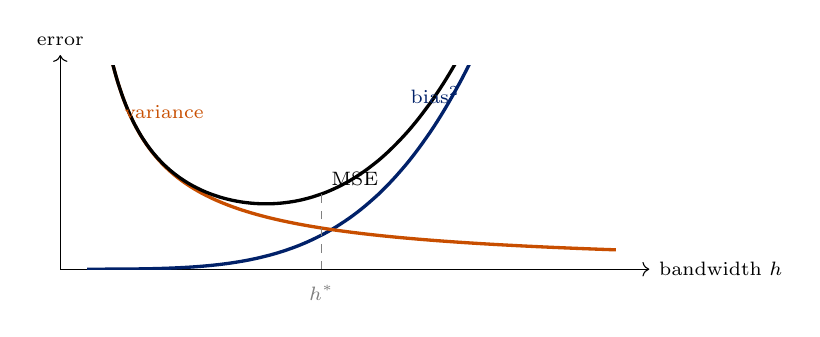
\begin{tikzpicture}[scale=0.85]
  \draw[->] (0,0) -- (8.8,0) node[right]{\scriptsize bandwidth $h$};
  \draw[->] (0,0) -- (0,3.2) node[above]{\scriptsize error};
  \begin{scope}
    \clip (0,0) rectangle (8.6,3.05);
    \draw[dukeblue,very thick,smooth,samples=90,domain=0.4:8.3,variable=\x] plot ({\x},{0.0022*\x*\x*\x*\x});
    \draw[accent,very thick,smooth,samples=90,domain=0.4:8.3,variable=\x] plot ({\x},{2.4/\x});
    \draw[black,very thick,smooth,samples=90,domain=0.4:8.3,variable=\x] plot ({\x},{0.0022*\x*\x*\x*\x+2.4/\x});
  \end{scope}
  \node[dukeblue] at (5.6,2.6) {\scriptsize bias$^2$};
  \node[accent] at (1.55,2.35) {\scriptsize variance};
  \node at (4.4,1.35) {\scriptsize MSE};
  \draw[gray,dashed] (3.9,0) -- (3.9,1.13);
  \node[gray] at (3.9,-0.35) {\scriptsize $h^{*}$};
\end{tikzpicture}
\end{center}
\vskip-10pt
\begin{itemize}\small\itemsep1pt
  \item \textbf{Wide} $h$: more data, lower variance, but the linear
        approximation is worse far from $c$ --- bias.
  \item \textbf{Narrow} $h$: less bias, but few observations --- variance.
  \item Choose $h$ by minimizing estimated MSE (Imbens--Kalyanaraman; the
        Calonico--Cattaneo--Titiunik version in \texttt{rdrobust}).
  \item \alert{The MSE-optimal bandwidth leaves a bias that invalidates the
        conventional interval.} Use the CCT \emph{robust bias-corrected}
        interval, which \texttt{rdrobust} reports by default.
\end{itemize}
\end{frame}
\begin{frame}[shrink=10]{Why the Optimal Bandwidth Breaks the Confidence Interval}
The local linear estimator has an asymptotic expansion
\begin{align*}
  \hat\tau_h - \tau \;\approx\; \underbrace{B\,h^2}_{\text{bias}}
  \;+\; \underbrace{O_p\big((nh)^{-1/2}\big)}_{\text{noise}} ,
\end{align*}
so squared bias grows like $h^4$ while variance falls like $1/(nh)$.
\vskip3pt
\begin{itemize}\itemsep3pt
  \item Minimizing MSE gives $h^{*} \propto n^{-1/5}$, at which the bias and the
        standard error are \alert{of the same order}.
  \item Consequently the conventional interval $\hat\tau_{h^*} \pm 1.96\,\hat{se}$
        is \emph{not} centred on $\tau$: it undercovers, sometimes badly.
  \item \srct{Calonico, Cattaneo, and Titiunik (2014)}: estimate the bias with a
        higher-order local polynomial, subtract it, and \alert{widen the interval
        to account for having estimated the bias}. That is the ``robust'' row in
        \texttt{rdrobust} output.
  \item \alert{Report the robust interval.} Reporting the conventional one at an
        MSE-optimal bandwidth is internally inconsistent.
\end{itemize}
\end{frame}

\begin{frame}[shrink=10]{Covariates, Power, and What to Report}
\begin{itemize}\itemsep3pt
  \item \textbf{Covariates are for precision only.} They must be
        \emph{pre-determined}, they should enter additively (not interacted with
        $D$), and the estimate should barely move when you add them. If it moves
        a lot, the design is in trouble, not improved
        \srcp{Calonico et al.\ 2019}.
  \item \textbf{Effective sample size}: report the number of observations
        \emph{inside the bandwidth} on each side. An RD with $n = 100{,}000$ often
        has 400 observations doing the work, and the standard errors should be
        read accordingly.
  \item \textbf{Power}: RD is a local method and is inherently data-hungry. The
        required sample size is a substantial multiple of an experiment's for the
        same power --- often quoted as around $3\times$, though the exact factor
        depends on the design --- because we are extrapolating to a boundary from
        one side at a time.
  \item \textbf{Discrete running variables and heaping}: rounded ages, coarse
        test-score grids, or income bunched at round numbers do not invalidate the
        design, but they do invalidate the continuous-$X$ asymptotics behind
        bandwidth selection and bias correction. Use a discrete-score method and
        say so.
\end{itemize}
\end{frame}



%%%%%%%%%%%%%%%%%%%%%%%%%%%%%%%%%%%%%%%%%%%%%%%%%%%%%%%%%%%%%%%%%%%%%%%%%%%%%%%
\section[Fuzzy RD]{Fuzzy RD}
%%%%%%%%%%%%%%%%%%%%%%%%%%%%%%%%%%%%%%%%%%%%%%%%%%%%%%%%%%%%%%%%%%%%%%%%%%%%%%%
\begin{frame}\sectionpage\end{frame}

\begin{frame}{When the Rule Is Not Followed}
Often crossing the cutoff changes the \emph{probability} of treatment rather than
determining it: eligibility is not take-up.
\begin{align*}
  \lim_{x\downarrow c}\Pr(D_i=1\mid X_i=x) - \lim_{x\uparrow c}\Pr(D_i=1\mid X_i=x)
  \ \in\ (0,1) .
\end{align*}
The fuzzy RD estimator is a ratio of two sharp RD estimates:
\begin{align*}
  \tau_{FRD} = \frac{\text{jump in } Y \text{ at } c}{\text{jump in } D \text{ at } c}
  = \frac{\lim_{x\downarrow c}\E[Y\mid x] - \lim_{x\uparrow c}\E[Y\mid x]}
         {\lim_{x\downarrow c}\E[D\mid x] - \lim_{x\uparrow c}\E[D\mid x]} .
\end{align*}
\vskip2pt
\begin{itemize}\itemsep2pt
  \item \alert{This is exactly the Wald estimator of Week 7}, with
        $\mathbf 1\{X\geq c\}$ as the instrument, estimated locally.
  \item The numerator alone is the \textbf{intention-to-treat} effect of crossing
        the cutoff, and it is worth reporting on its own --- it needs no
        first-stage assumption.
\end{itemize}
\end{frame}

\begin{frame}[shrink=10]{Fuzzy RD Inherits Everything From IV}
\begin{itemize}\itemsep3pt
  \item \textbf{Exclusion}: crossing the cutoff must affect $Y$ only through $D$.
        If the threshold also triggers something else --- a different school, a
        different caseworker, a label --- exclusion fails.
  \item \textbf{Monotonicity}: no one is treated \emph{because} they fell below
        the cutoff.
  \item \textbf{The estimand is doubly local}: the effect for \alert{compliers at
        the cutoff}. Not the ATE, not the ATT, and not the effect for everyone
        near the cutoff.
  \item \textbf{Weak first stage} is a real risk: if take-up jumps by only a few
        percentage points, you are dividing by a small noisy number and all the
        Week 7 pathologies return. Report the size of the jump in $D$.
\end{itemize}
\vskip3pt
\begin{block}{Related designs}
\textbf{Regression kink}: identification from a change in \emph{slope} rather
than level. \textbf{Geographic RD}: the running variable is distance to a
boundary, and the ``cutoff'' is two-dimensional. \textbf{Multi-cutoff RD}:
different units face different thresholds, which can be normalized and pooled.
\end{block}
\end{frame}

%%%%%%%%%%%%%%%%%%%%%%%%%%%%%%%%%%%%%%%%%%%%%%%%%%%%%%%%%%%%%%%%%%%%%%%%%%%%%%%
\section[Validity]{Validity}
%%%%%%%%%%%%%%%%%%%%%%%%%%%%%%%%%%%%%%%%%%%%%%%%%%%%%%%%%%%%%%%%%%%%%%%%%%%%%%%
\begin{frame}\sectionpage\end{frame}

\begin{frame}{The Threat: Manipulation}
Continuity fails if units can \emph{precisely} control which side of the cutoff
they land on --- retaking a test until you pass, reporting income just under a
threshold, a firm holding hiring just below a regulatory headcount.
\vskip3pt
\begin{itemize}\itemsep3pt
  \item \alert{Imprecise control is fine.} \srct{Lee (2008)}'s insight is that if
        agents cannot control $X$ to the last decimal, assignment near the cutoff
        is as good as random even though agents influence $X$.
  \item \textbf{Density test} \srcp{McCrary 2008; Cattaneo, Jansson, and Ma 2020}:
        is the density of $X$ continuous at $c$? A spike on the advantaged side is
        direct evidence of sorting.
  \item \textbf{Covariate smoothness}: run the RD with \emph{pre-determined
        covariates} as outcomes. They should show no jump. This is the single
        most persuasive check, and it is the RD analogue of a balance table.
  \item \textbf{Donut hole}: drop observations immediately around $c$, where
        manipulation would concentrate, and see whether the estimate survives.
\end{itemize}
\end{frame}

\begin{frame}{Other Checks and Common Errors}
\begin{itemize}\itemsep3pt
  \item \textbf{Placebo cutoffs}: estimate at fake thresholds away from $c$, using
        only data on one side so the real discontinuity is not picked up.
        Significant ``effects'' there mean your procedure finds jumps everywhere.
  \item \textbf{Bandwidth sensitivity}: plot $\hat\tau$ against $h$ over a wide
        range with robust intervals. A result that exists only at one bandwidth is
        not a result.
  \item \alert{Do not use a high-order global polynomial}
        \srcp{Gelman and Imbens 2019}. The implied weights on distant
        observations are large, oscillating, and indefensible; estimates wander
        with the degree.
  \item \alert{Do not control for post-treatment covariates}, and do not interact
        covariates with $D$ unless you mean to estimate heterogeneity.
  \item \alert{Do not report only the conventional interval} at an MSE-optimal
        bandwidth.
\end{itemize}
\end{frame}

\begin{frame}{Reading and Reporting an RD}
\begin{enumerate}\itemsep2pt
  \item \textbf{The picture first.} Binned means of $Y$ against $X$, with the
        fitted local polynomials and the cutoff. If the jump is not visible, be
        sceptical of the number.
  \item The bandwidth, how it was chosen, and the effective $n$ on each side.
  \item Robust bias-corrected confidence intervals.
  \item The density test and the covariate-smoothness checks.
  \item A bandwidth-sensitivity plot and placebo cutoffs.
  \item For fuzzy designs, the size of the jump in treatment take-up, and the
        intention-to-treat effect alongside.
  \item An explicit statement that the estimand is local to the cutoff.
\end{enumerate}
\end{frame}

\begin{frame}{Looking Ahead}
\begin{itemize}\itemsep4pt
  \item RD buys extraordinary credibility at the cost of a very local estimand.
        The identifying variation is visible in a scatterplot, and the main
        threats --- sorting, bandwidth dependence --- are checkable.
  \item Note the family resemblance: sharp RD is a local experiment; fuzzy RD is
        local IV. The tools recombine rather than multiply.
  \item \textbf{Next week}: designs that use variation over \emph{time} rather
        than across a threshold.
  \item Note again how the estimand was chosen by the design rather than by us.
        Saying so plainly is part of reporting an RD honestly.
\end{itemize}
\vskip4pt
\begin{block}{Problem Set 4}
Assigned today, due Monday November 2. Covers Weeks 7 and 9.
\end{block}
\end{frame}

\begin{frame}[allowframebreaks]{References}
\footnotesize
\begin{itemize}\itemsep3pt
\item Calonico, Sebastian, Matias D. Cattaneo, and Roc\'{\i}o Titiunik. 2014.
``Robust Nonparametric Confidence Intervals for Regression-Discontinuity
Designs.'' \textit{Econometrica} 82(6): 2295--2326.
\item Calonico, Sebastian, Matias D. Cattaneo, Max H. Farrell, and
Roc\'{\i}o Titiunik. 2019. ``Regression Discontinuity Designs Using Covariates.''
\textit{Review of Economics and Statistics} 101(3): 442--451.
\item Cattaneo, Matias D., Michael Jansson, and Xinwei Ma. 2020. ``Simple Local
Polynomial Density Estimators.'' \textit{Journal of the American Statistical
Association} 115(531): 1449--1455.
\item Gelman, Andrew and Guido Imbens. 2019. ``Why High-Order Polynomials Should
Not Be Used in Regression Discontinuity Designs.'' \textit{Journal of Business \&
Economic Statistics} 37(3): 447--456.
\item Hahn, Jinyong, Petra Todd, and Wilbert van der Klaauw. 2001.
``Identification and Estimation of Treatment Effects with a
Regression-Discontinuity Design.'' \textit{Econometrica} 69(1): 201--209.
\item Imbens, Guido W. and Thomas Lemieux. 2008. ``Regression Discontinuity
Designs: A Guide to Practice.'' \textit{Journal of Econometrics} 142(2): 615--635.
\item Imbens, Guido W. and Karthik Kalyanaraman. 2012. ``Optimal Bandwidth Choice
for the Regression Discontinuity Estimator.'' \textit{Review of Economic Studies}
79(3): 933--959.
\item Lee, David S. 2008. ``Randomized Experiments from Non-Random Selection in
U.S. House Elections.'' \textit{Journal of Econometrics} 142(2): 675--697.
\item Lee, David S. and Thomas Lemieux. 2010. ``Regression Discontinuity Designs
in Economics.'' \textit{Journal of Economic Literature} 48(2): 281--355.
\item McCrary, Justin. 2008. ``Manipulation of the Running Variable in the
Regression Discontinuity Design: A Density Test.'' \textit{Journal of
Econometrics} 142(2): 698--714.
\end{itemize}
\end{frame}

\end{document}
